\documentclass{article}
\usepackage{tikz}
\usepackage{amsmath,amssymb}
\usetikzlibrary{arrows.meta, calc, backgrounds}

\begin{document}

\begin{figure}[htbp]
  \centering
  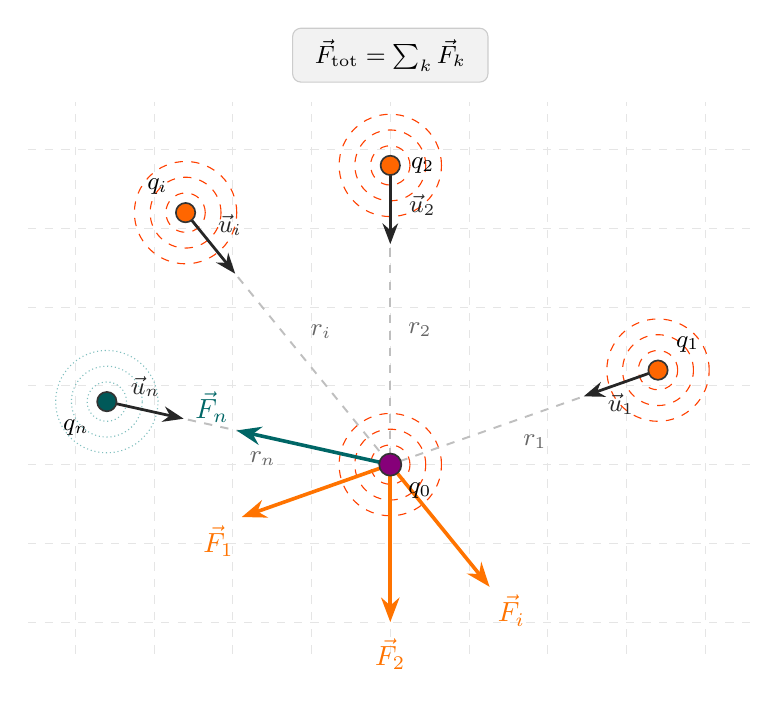
\begin{tikzpicture}[>=Stealth, font=\small\sffamily]

    % Stili grafici
    \tikzset{
      gridline/.style={draw=gray!20, line width=0.3pt, dashed},
      badge/.style={draw=gray!40, fill=gray!10, rounded corners=3pt, inner xsep=8pt, inner ysep=4pt, font=\small\sffamily},
      forcearrow/.style={line width=1.3pt, ->},
      posline/.style={draw=gray!50, line width=0.7pt, dashed},
      unitarrow/.style={line width=1.0pt, ->, color=black!85}
    }

    % Griglia tecnica di sottofondo
    \draw[gridline] (-4.6,-2.4) grid (4.6,4.6);

    % Coordinate dei centri di carica
    \coordinate (q0) at (0,0);
    \coordinate (q1) at (3.4, 1.2);
    \coordinate (q2) at (0.0, 3.8);
    \coordinate (qi) at (-2.6, 3.2);
    \coordinate (qn) at (-3.6, 0.8);

    % Anelli concentrici attorno alle cariche
    \foreach \r in {0.25, 0.45, 0.65} {
      \draw[orange!50!red, line width=0.4pt, dashed] (q0) circle (\r);
      \draw[orange!50!red, line width=0.4pt, dashed] (q1) circle (\r);
      \draw[orange!50!red, line width=0.4pt, dashed] (q2) circle (\r);
      \draw[orange!50!red, line width=0.4pt, dashed] (qi) circle (\r);
      \draw[teal!50, line width=0.4pt, densely dotted] (qn) circle (\r);
    }

    % Congiungenti tratteggiate
    \draw[posline] (q1) -- (q0);
    \draw[posline] (q2) -- (q0);
    \draw[posline] (qi) -- (q0);
    \draw[posline] (qn) -- (q0);

    % Distanze r_k
    \node[below right=1pt, font=\small\itshape, color=gray!80!black] at ($(q1)!0.55!(q0)$) {$r_1$};
    \node[right=3pt, font=\small\itshape, color=gray!80!black] at ($(q2)!0.55!(q0)$) {$r_2$};
    \node[above right=1pt, font=\small\itshape, color=gray!80!black] at ($(qi)!0.55!(q0)$) {$r_i$};
    \node[below=2pt, font=\small\itshape, color=gray!80!black] at ($(qn)!0.55!(q0)$) {$r_n$};

    % Versori u_k lungo le congiungenti
    \draw[unitarrow] ($(q1)!0cm!(q0)$) -- ($(q1)!1cm!(q0)$) node[midway, below=0 pt, font=\bfseries\small] {$\vec{u}_1$};
    \draw[unitarrow] ($(q2)!0cm!(q0)$) -- ($(q2)!1cm!(q0)$) node[midway, right=3pt, font=\bfseries\small] {$\vec{u}_2$};
    \draw[unitarrow] ($(qi)!0cm!(q0)$) -- ($(qi)!1cm!(q0)$) node[midway, above right=-1pt, font=\bfseries\small] {$\vec{u}_i$};
    \draw[unitarrow] ($(qn)!0cm!(q0)$) -- ($(qn)!1cm!(q0)$) node[midway, above=1pt, font=\bfseries\small] {$\vec{u}_n$};

    % Vettori forza applicati alla carica sonda q0
    \draw[forcearrow, color=orange!90!red] (q0) -- ($(q0)!-2.0cm!(q1)$) node[below left=-1pt, font=\bfseries] {$\vec{F}_1$};
    \draw[forcearrow, color=orange!90!red] (q0) -- ($(q0)!-2.0cm!(q2)$) node[below=2pt, font=\bfseries] {$\vec{F}_2$};
    \draw[forcearrow, color=orange!90!red] (q0) -- ($(q0)!-2.0cm!(qi)$) node[below right=-1pt, font=\bfseries] {$\vec{F}_i$};
    \draw[forcearrow, color=teal!80!black] (q0) -- ($(q0)!2.0cm!(qn)$) node[above left=-1pt, font=\bfseries] {$\vec{F}_n$};

    % Particelle cariche
    \filldraw[fill=orange!80!red, draw=black!80, line width=0.6pt] (q1) circle (3.5pt);
    \node[above right=3pt, font=\small\bfseries] at (q1) {$q_1$};

    \filldraw[fill=orange!80!red, draw=black!80, line width=0.6pt] (q2) circle (3.5pt);
    \node[right=4pt, font=\small\bfseries] at (q2) {$q_2$};

    \filldraw[fill=orange!80!red, draw=black!80, line width=0.6pt] (qi) circle (3.5pt);
    \node[above left=3pt, font=\small\bfseries] at (qi) {$q_i$};

    \filldraw[fill=teal!70!black, draw=black!80, line width=0.6pt] (qn) circle (3.5pt);
    \node[below left=3pt, font=\small\bfseries] at (qn) {$q_n$};

    \filldraw[fill=purple!70!blue, draw=black!80, line width=0.6pt] (q0) circle (4.0pt);
    \node[below right=3pt, font=\small\bfseries] at (q0) {$q_0$};

    % Badge superiore esplicativo
    \node[badge] at (0, 5.2) {$\vec{F}_{\mathrm{tot}} = \sum_{k} \vec{F}_k$};

  \end{tikzpicture}
  \caption{Principio di sovrapposizione per le forze elettrostatiche agenti sulla carica di prova $q_0$.}
  \label{fig:sovrapposizione_infografica}
\end{figure}

\end{document}